\section{Experiments}
\label{sec:experiments}
We evaluate TSD along the three axes introduced above: reference medium,
requested subject, and reference-layout retention. The initial study tests
both task regimes against the native editor on 40 references. An expanded
study adds multiple prompts, dedicated style-transfer methods, and stronger
same-backbone guidance controls. We then examine how latent interventions
change the balance between style and subject fidelity.

\subsection{Experimental setup}
\label{sec:setup}
\paragraph{Initial and expanded studies.}
The initial study uses 40 style references with the prompt ``a panda eating
bamboo'' and seed 65. It compares the original semantic and global TSD
configurations with native editing instructions that respectively request
reference-layout retention and a new composition. We retain its stored
measurements as a distinct study. The expanded study uses newly generated
outputs with recorded configurations and input/output hashes.

The new reference collection contains 48 public Krea-generated images across
eight medium categories. We selected references for medium clarity, visual
quality, and diversity before inspecting generated outputs. Each category
contributes one development and five test references, giving an 8/40 split.
Every method receives the same RGB $512\times512$ reference, obtained by
aspect-preserving resizing and center cropping of the public 1024-pixel
source version. Six fixed prompts request a panda, castle, cat, sunflower
field, fisherman portrait, and lighthouse. Source identifiers, transforms,
and image hashes are provided in the supplementary records. The completed
expanded comparison uses the eight development references and seed 64.
The 40 disjoint references are reserved for the multi-seed test protocol
in Sec.~\ref{sec:expanded}.

\paragraph{Comparison methods.}
The common task supplies a style reference and target text. TSD and
reference CFG share the frozen Klein-9B-base backbone, text CFG 4, and the
same transfer instruction. The reference-CFG baseline is chosen from a
development sweep of guidance strengths and sampling budgets. Its retained
setting uses 72 intervals and reference scale $\gamma=5$.
Attention Distillation (AD) uses SD1.5 with 50 steps, two inner updates,
learning rate .015, text CFG 7.5, and AdaIN
\citep{zhou2025attentiondistillation}. USO uses its style-only interface
with FLUX.1-dev, pretrained rank-128 adapters and SigLIP features, 25 steps,
and guidance 4 \citep{wu2025uso}. USO stores weights in FP8 with bf16
computation. Backbones, pretrained adapters, and precision are recorded
alongside the method settings. StyleShot uses its pretrained SD1.5
style encoder and adapter with style scale 1, text CFG 7.5, and the official
float32 pipeline \citep{gao2024styleshot}. Its nominal 50-step PNDM schedule
performs 51 UNet evaluations. InstantStyle uses the official style-block
IP-Adapter interface on SDXL, with 30 Euler steps, text CFG 5, style scale
1, and float16 inference \citep{wang2024instantstyle}. Its image condition
enters the designated style block. Quality and negative prompts follow
the official example and are recorded in the supplement.

\paragraph{Metrics and paired analysis.}
We report CSD reference--output similarity for style
\citep{somepalli2024csd}, CLIP ViT-B/32 image--text similarity to the literal
content request \citep{radford2021clip}, and DINOv2 ViT-B/14 reference-layout
similarity \citep{oquab2024dinov2}. For normalized patch features $P_x$,
let $q_x=\operatorname{vec}_{\rm off}(P_xP_x^\top)$. The layout measure is
\begin{equation}
\Lambda(x,r)=\operatorname{corr}(q_x,q_r).
\label{eq:layout}
\end{equation}
Higher $\Lambda$ indicates more similar spatial self-similarity structure,
which can be useful for semantic editing. Both geometry and shared
semantics can affect this readout. We compute method differences on matched
reference/prompt/seed cells and bootstrap reference groups with all their
repeated observations together, using 10,000 resamples.

\subsection{Full benchmark against the frozen model's native edit}
\label{sec:initialresults}
The same frozen model's native image-and-text editing path provides the
initial baseline. In TSD, the reference enters the score-contrast objective
while the reverse solver itself uses the reference-free branch. Setting the
contrast to zero therefore gives text-only sampling, rather than native
image editing. The native keep-layout and new-layout instructions are
separate reference-conditioned comparisons.

The initial study tests whether one operator can strengthen the reference
medium under both composition objectives. Table~\ref{tab:benchmark} retains
the original 160 measurements, with sample SD across the 40 references.
The table summarizes the stored measurements from the initial study.
Its complete per-reference records appear in the supplement.

\begin{table}[t]
\centering\small
\caption{Initial 40-reference study, one content prompt and seed 65.
Values are mean $\pm$ sample SD across references. S/G are the original
semantic/global configurations. Layout measures retention of reference
structure, whose desired level depends on the task.}
\label{tab:benchmark}
\resizebox{\columnwidth}{!}{\begin{tabular}{lccc}
\toprule
Method & CSD $\uparrow$ & CLIP-T $\uparrow$ & Layout \\
\midrule
TSD-S (semantic) & 0.719 $\pm$ 0.079 & 0.295 $\pm$ 0.031 & 0.572 $\pm$ 0.148 \\
TSD-G (global) & 0.615 $\pm$ 0.096 & 0.304 $\pm$ 0.027 & 0.414 $\pm$ 0.109 \\
Native keep-layout & 0.267 $\pm$ 0.165 & 0.319 $\pm$ 0.012 & 0.317 $\pm$ 0.073 \\
Native new-layout & 0.247 $\pm$ 0.157 & 0.315 $\pm$ 0.011 & 0.299 $\pm$ 0.065 \\
\bottomrule
\end{tabular}
}
\end{table}

TSD-S increases mean CSD from .267 to .719 relative to native keep-layout
editing, and TSD-G increases it from .247 to .615 relative to native
new-layout editing. Every reference has a positive paired CSD difference
in both comparisons. CLIP-T decreases from .319 to .295 and from .315 to
.304, respectively. The two TSD configurations also differ in layout
retention: .572 for S and .414 for G. Thus the original study supports two
useful operating regimes, with stronger reference matching accompanied by
different amounts of reference structure.

CLIP-T is read against the literal content request, separately from the
style-transfer instruction. The earlier five-reference, four-additional-prompt
study is retained in the supplement using its stored prompt-level summaries.
The new multi-prompt comparison below has its own inputs and measurements.

The style increase must be interpreted together with composition. Against
each output's paired native baseline, only 1/40 semantic and 3/40 global
outputs have no greater layout similarity. The full-set CSD gains therefore
do not by themselves establish a style advantage at matched layout. The
expanded study below evaluates this condition explicitly and includes a
swept reference-guidance control.

\subsection{Expanded reference-plus-text comparison}
\label{sec:results}
We select TSD settings and direct-reference controls on a 16-cell grid of
four references, two prompts, and two seeds. The resulting 25-configuration
study contains 400 outputs. We then compare the retained settings, AD, USO,
StyleShot, and InstantStyle on all eight development references and six prompts at seed
64, giving 48 paired inputs per method. Table~\ref{tab:coverage} reports all
336 outputs in this comparison. The supplementary material gives the full
configuration study, including exact reused cells.

\begin{table}[t]
\centering\small
\caption{Development coverage on eight references, six prompts, and seed
64 (48 outputs per row). Layout measures reference-layout retention.
Backbones and precision are specified in the setup.}
\label{tab:coverage}
\resizebox{\columnwidth}{!}{\begin{tabular}{lrrr}
\toprule
Method & CSD $\uparrow$ & CLIP-T $\uparrow$ & Layout \\
\midrule
Reference CFG, 72/$\gamma=5$ & 0.3190 & 0.3005 & 0.3118 \\
AD (SD1.5) & 0.7069 & 0.2692 & 0.3224 \\
USO (FLUX.1, FP8) & 0.4117 & 0.3178 & 0.2953 \\
StyleShot (SD1.5) & 0.5042 & 0.2840 & 0.2703 \\
InstantStyle (SDXL) & 0.4947 & 0.2616 & 0.2900 \\
TSD, 8/K5 & 0.4291 & 0.3078 & 0.3101 \\
TSD, 25/K2 & 0.5751 & 0.2982 & 0.3503 \\
\bottomrule
\end{tabular}
}
\end{table}

\begin{figure*}[t]
\centering
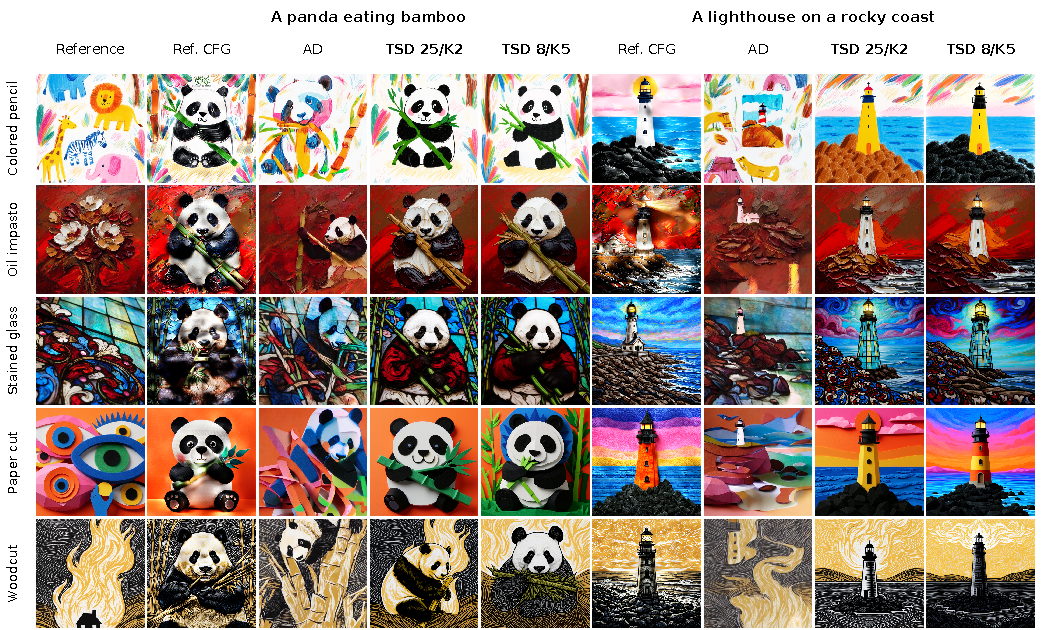
\includegraphics[width=\textwidth]{two_prompt_comparison.pdf}
\caption{Reference-guided generation across two content prompts and five media.
Each row shares a reference. Each prompt block compares reference CFG,
Attention Distillation, and two TSD settings on the same input and seed 64.
TSD preserves characteristic color, material, and surface patterns across
the two subjects. The 25/K2 and 8/K5 settings change the strength and spatial
expression of the reference signal. These outputs belong to the expanded
development comparison in Table~\ref{tab:coverage}.}
\label{fig:twoprompt}
\end{figure*}

Both TSD settings strengthen style matching over the selected reference-CFG
baseline. TSD8/K5 raises mean CSD from .3190 to .4291 and CLIP-T from .3005
to .3078. The paired differences are .1101 for CSD (reference-group 95\%
bootstrap interval $[.0720,.1463]$) and .0073 for CLIP-T
($[.0004,.0157]$). Its mean layout similarity is .3101, compared with .3118
for the direct control. TSD25/K2 further increases CSD to .5751, with
CLIP-T .2982 and layout similarity .3503. Its paired CSD increase over
reference CFG is .2561 ($[.2178,.2940]$).

The dedicated methods place these settings in a broader style--subject
comparison. Relative to AD, TSD25/K2 has higher CLIP-T by .0291
($[.0233,.0354]$) and lower CSD by .1319 ($[.0559,.2049]$ for AD minus TSD).
Relative to USO, it has higher CSD by .1633 ($[.0876,.2506]$) and lower
CLIP-T by .0195 ($[.0149,.0249]$ for USO minus TSD). TSD8/K5 favors subject
alignment within our two settings, while TSD25/K2 strengthens the style
signal. StyleShot obtains CSD .5042 and CLIP-T .2840, compared with .5751 and
.2982 for TSD25/K2. InstantStyle obtains CSD .4947 and CLIP-T .2616. These development
comparisons use eight reference groups.

Figure~\ref{fig:twoprompt} shows how the reference signal appears in different
media and subjects. In stained glass, TSD carries colored panes and dark
outlines into both the panda and lighthouse. The paper-cut examples retain
layered shapes, while the oil-paint examples reproduce broad impasto strokes.
The two TSD settings also differ visibly in framing and surface treatment.
These examples complement the joint metric readout: medium transfer and
reference-layout retention are related properties, but neither is a
substitute for rendering the target subject.

\paragraph{Paired layout constraint.}
We also evaluate style differences on cells whose TSD output retains no
more layout than its corresponding baseline output:
\begin{equation}
\mathcal I=\{i:\Lambda(x_i^{\rm TSD},r_i)
\leq\Lambda(x_i^{\rm baseline},r_i)\}.
\label{eq:pairedconstraint}
\end{equation}
Against reference CFG, TSD8/K5 satisfies this condition on 22/48 cells.
Within this subset, its mean CSD and CLIP-T differences are .0867 and .0041.
TSD25/K2 satisfies the condition on 18/48 cells, with differences .2127
and $-.0045$. We report these descriptive subset results together with their
coverage and the complete-grid comparison.

\subsection{The style-locality axis and ablations}
\label{sec:interventioncontrols}
\paragraph{Why use a moderate update count?}
At a fixed 25-step solver, learning rate .01, and target offset .05,
K1/K2/K5 produce CSD .3726/.5555/.7302 and CLIP-T
.3109/.3110/.2796 on the same 16-cell search grid. K2 strengthens style
relative to K1 while retaining a similar subject score, and uses 146 DiT
forwards compared with 290 for K5. This motivates the retained 25/K2
setting. Reducing the K5 learning rate to .005 instead gives CSD .6288 and
CLIP-T .2986. Update count and learning rate therefore provide different
style--subject operating points.

\paragraph{Sampling and intervention location.}
The common-node controls insert $\{.8,.6,.4,.2\}$ and perform one update
at each positive node. This fixes guidance locations and counts across
nominal solver lengths. The dense configurations intervene at the original
positive solver nodes. We record actual intervals, optimizer choice,
update count, and displacement for each configuration. The complete search
also includes RMS-SGD and shorter reference-guidance controls. At the four
shared nodes, nominal 25-step and eight-step sampling yield CSD
.0386/.0315 and CLIP-T .3190/.3168, respectively. Both have much lower
style similarity than the dense interventions in this study. These
measurements show the importance of the intervention schedule alongside
solver resolution. This design
compares discretization with matched intervention locations. The dense
8/K5 and 25/K2 settings instead change several factors together and define
operating points rather than an isolated effect of reverse-step count.

\paragraph{Model calls and timing.}
TSD8/K5 and TSD25/K2 use 86/146 DiT forwards and 35/48 latent backward
calls respectively. The backward calls differentiate the detached-target
loss. Reference CFG uses 288 DiT forwards, AD uses 200 UNet forwards, and
USO uses 25 DiT forwards under their respective settings. StyleShot uses
51 UNet forwards. Calls from
different backbones describe different computations. A common-hardware
timing comparison is reserved below.
End-to-end timing includes reference/text encoding, sampling, latent
optimization, and output decoding. Model loading is measured separately,
and single- and two-GPU placements are grouped separately in cost records.

\pendingexperiment{Inference cost}{Complete the same-hardware comparison
of end-to-end latency, peak allocated memory, precision, and offload policy.
Separate single- and two-GPU placements and report model loading separately.
The measured model-call counts above remain part of the completed analysis.}

\subsection{Multi-seed comparison}
\label{sec:expanded}
The held-out protocol uses 40 disjoint test references, six target prompts,
and seeds 64/65/66, giving 720 reference/prompt/seed cells per configuration.
The first frozen matrix contains reference CFG, AD, USO, and two TSD
settings, or 3,600 outputs. A separately validated extension adds StyleShot,
InstantStyle, and CSGO on the same inputs. The final comparison thus reserves
six baselines and two TSD settings, with a planned total of 5,760 outputs.
Table~\ref{tab:heldoutpending} provides the result slots. No test result is
used to select the method settings.

\begin{table}[t]
\centering\small
\caption{Held-out comparison, results pending. Each row has a planned
720 cells on the same 40-reference, six-prompt, three-seed grid. TBD denotes
an unfilled result, including rows whose generation may already be complete.}
\label{tab:heldoutpending}
\begin{tabular}{lccc}
\toprule
Method & CSD $\uparrow$ & CLIP-T $\uparrow$ & Layout \\
\midrule
Reference CFG & \pendingcell & \pendingcell & \pendingcell \\
AD & \pendingcell & \pendingcell & \pendingcell \\
USO & \pendingcell & \pendingcell & \pendingcell \\
StyleShot & \pendingcell & \pendingcell & \pendingcell \\
InstantStyle & \pendingcell & \pendingcell & \pendingcell \\
CSGO & \pendingcell & \pendingcell & \pendingcell \\
\midrule
TSD 8/K5 & \pendingcell & \pendingcell & \pendingcell \\
TSD 25/K2 & \pendingcell & \pendingcell & \pendingcell \\
\bottomrule
\end{tabular}

\end{table}

\pendingexperiment{Held-out results}{Complete generation, metric evaluation,
and reference-group paired intervals for the original matrix and validated
baseline extension. Fill Table~\ref{tab:heldoutpending}, followed by the
paired layout-constrained analysis and per-medium comparison.}

\subsection{Perceptual evaluation}
\label{sec:human}
The planned blinded study pairs TSD25/K2 with each of the six baselines on
40 fixed reference/prompt/seed cases. Each pair is assigned three independent
human judgments. The target is 240 pairs and 720 judgments, with separate
questions on style, subject, and overall preference. The displayed method
names are hidden and left/right positions are randomized. The supplementary
protocol specifies sampling and uncertainty estimation.

\pendingexperiment{Human preferences}{Collect the planned judgments and
report actual participant and response counts, wins, ties, unavailable
responses, and reference/rater-aware uncertainty. Overall preference is the
primary readout. No human preference result is available in this draft.}
